\documentclass{beamer}

\usepackage{../macros}

\usepackage{fontspec}
\newfontfamily\arabicfont{Damascus}
\newfontfamily\myanmarfont{Myanmar Sangam MN}
\newfontfamily\devanagarifont{Devanagari Sangam MN}
\newfontfamily\bengalifont{Bangla MN}
\newfontfamily\gurumukhifont{Gurmukhi MN}

\makeatletter
\long\def\pgfshapeaddanchor#1#2{%
{%
  \def\pgf@sm@shape@name{#1}%
  \let\anchor=\pgf@sh@anchor%
  #2}%
}
\pgfshapeaddanchor{rectangle}{%
  \anchor{north north west}{%
    \pgf@process{\southwest}%
    \pgf@xa=1.5\pgf@x%
    \pgf@process{\northeast}%
    \pgf@x.5\pgf@x%
    \advance\pgf@x by \pgf@xa%
    \pgf@x=.25\pgf@x%
  }%
}
\makeatother

\title{Numbers}

\begin{document}

\frame{
  \titlepage
}

\begin{frame}{Computers and Data abstraction}
  \begin{block}{}
    \begin{itemize}
      \item An old history
      \item Abstraction remains abstractions
      \item How to make by itself?
    \end{itemize}
  \end{block}
\end{frame}

\begin{frame}{Counting}
  \begin{block}{}
    Soon after language develops, it is safe to assume that humans begin counting to represent amount of cows, volume of wine, area of fields, \dots
    
    It is safe to assume too that fingers and thumbs provide nature’s abacus
  \end{block}
  
  \hfill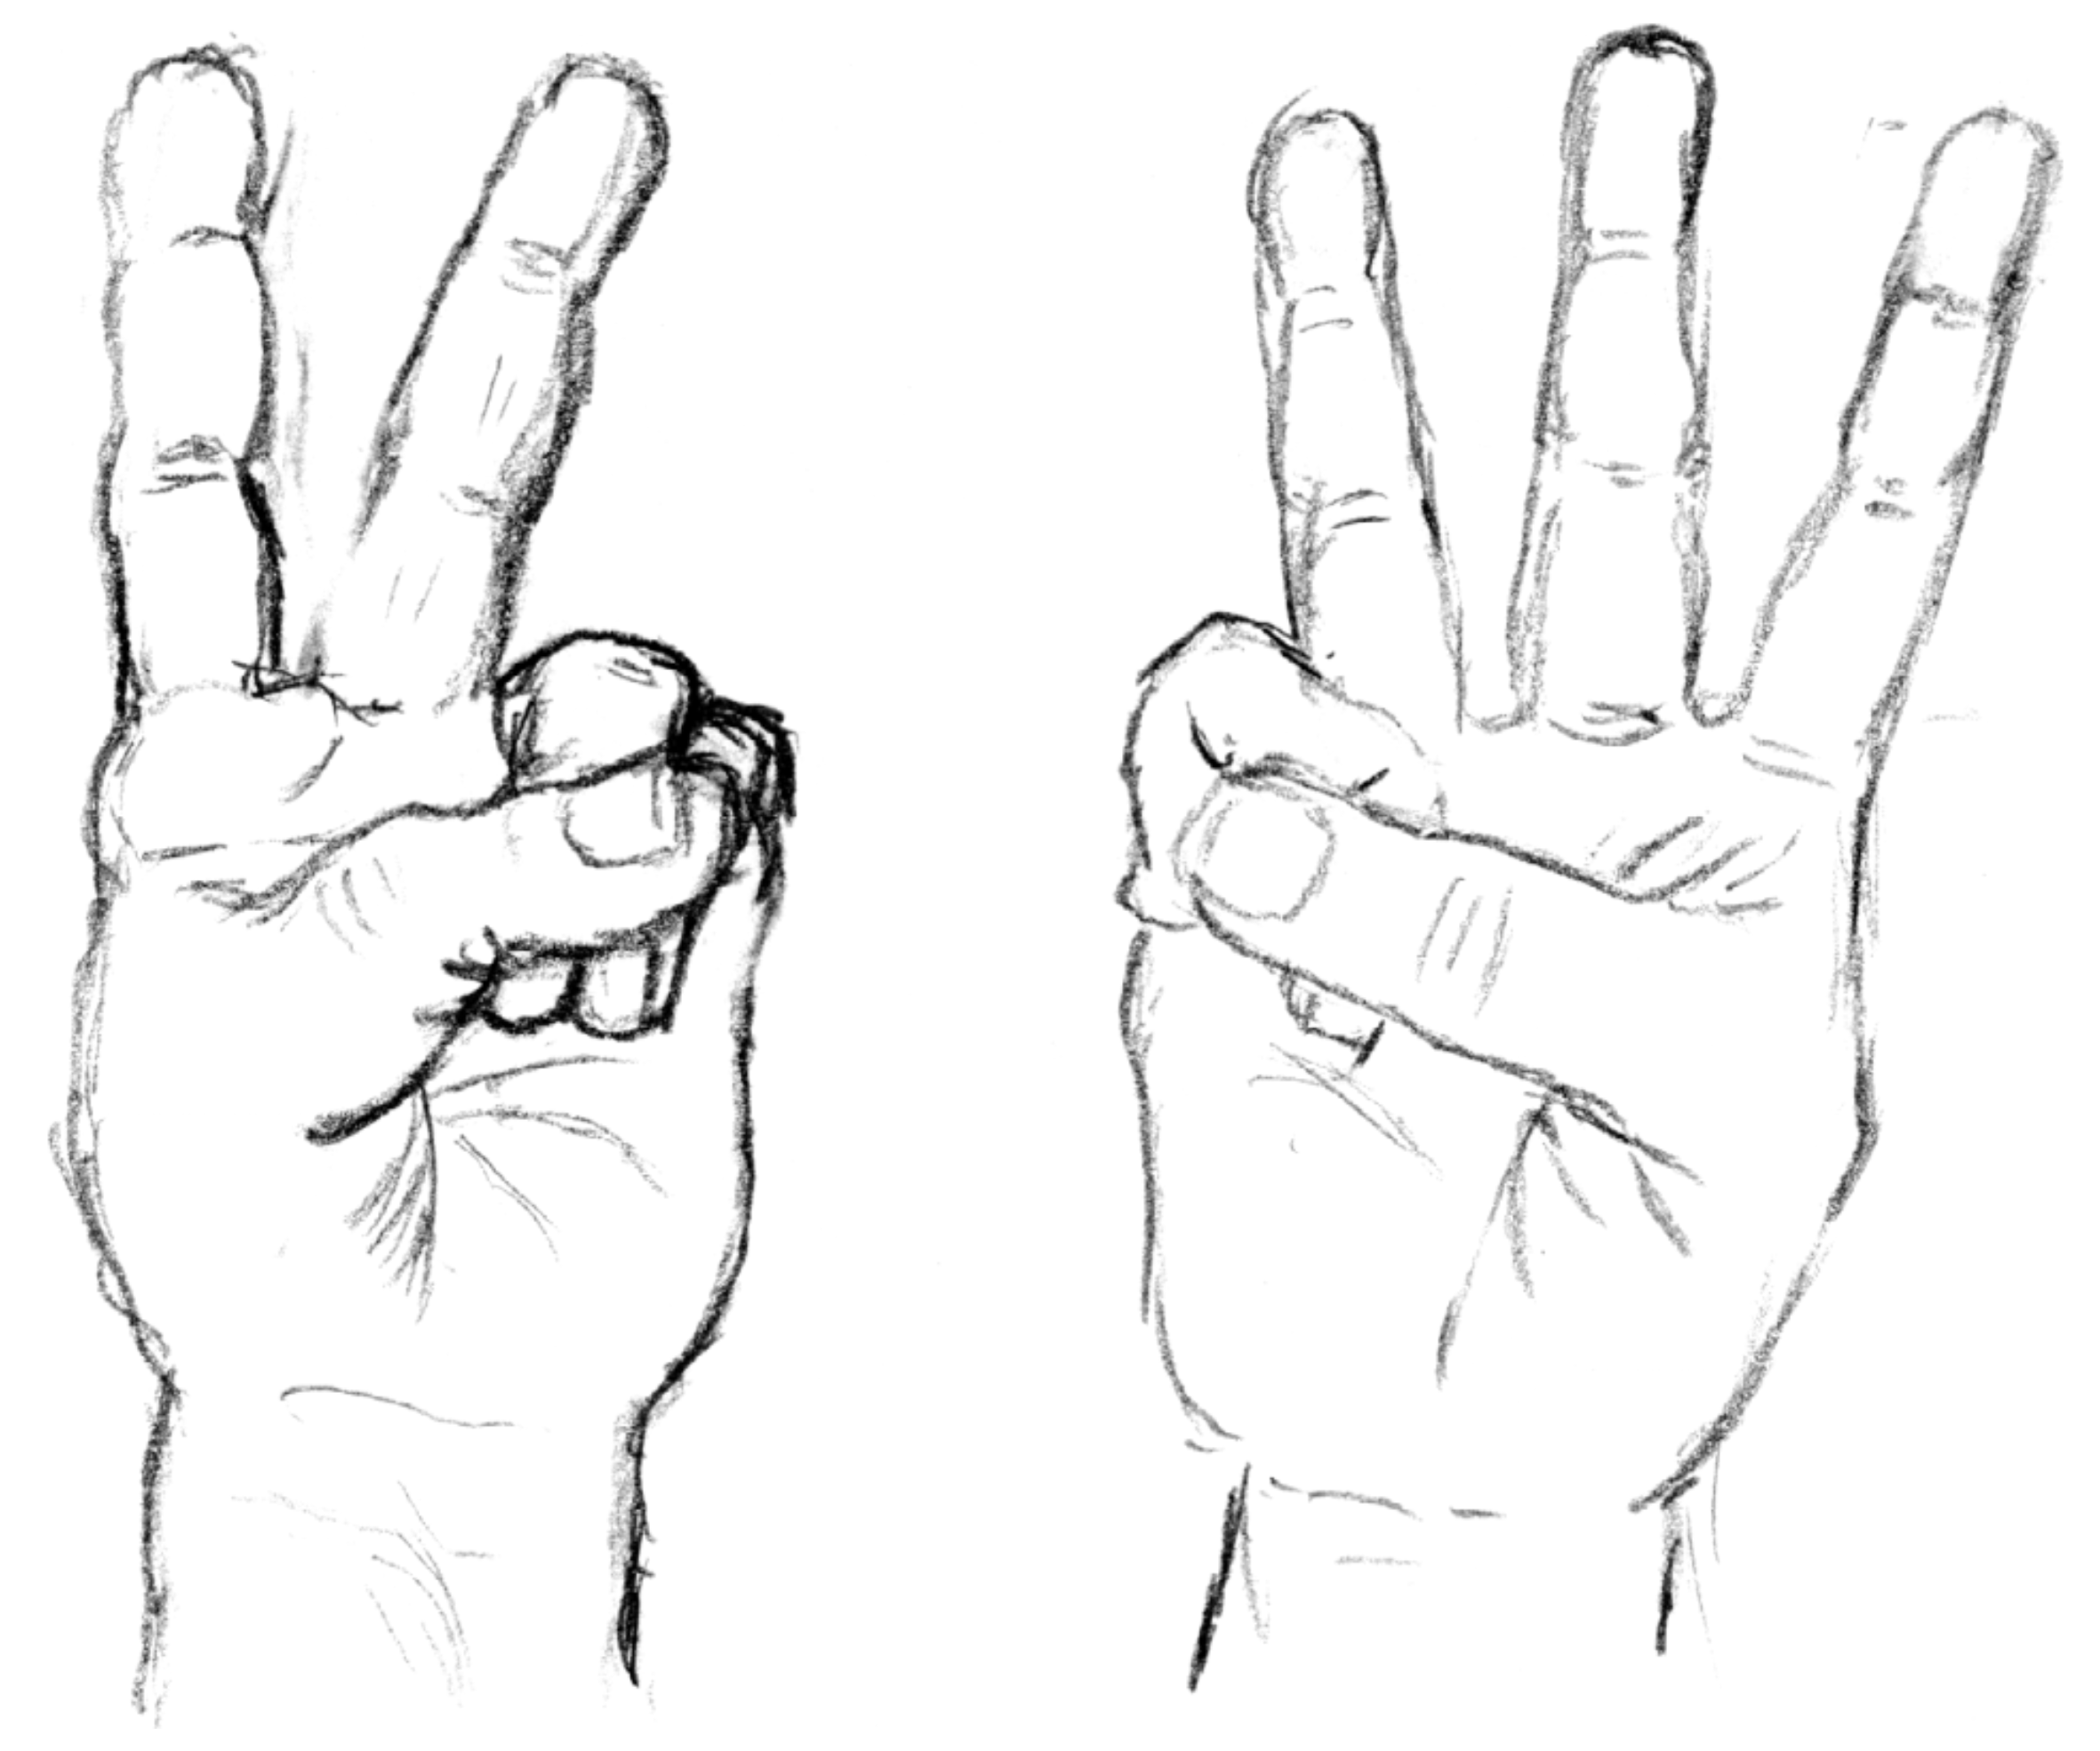
\includegraphics[width=0.25\linewidth]{compter.png}\hfill\includegraphics[width=0.25\linewidth]{abaque.png}\hfill~
  
  \begin{remark}
    \begin{itemize}
      \item The decimal and duodecimal systems are no accidents, ten and twelve have been the bases of most counting systems in history
      \item Abacus from greek ``dust table" is the generic name given to ``planar mechanical instrument" for computation and counting
    \end{itemize}
  \end{remark}
\end{frame}

\begin{frame}{Modern numbers}
  \begin{block}{}
    Arab numbers (and 10 basis digit system) are a modern representation (4th century)
    
    \begin{center}\small
      \begin{tabular}{l *{10}{c}}
       & 0 &1 & 2 & 3 & 4 & 5 & 6 & 7 & 8 & 9\\
      Arabic & {\arabicfont ٠} & {\arabicfont ١} & {\arabicfont ٢} & {\arabicfont ٣} & {\arabicfont ٤} & {\arabicfont ٥} & {\arabicfont ٦} & {\arabicfont ٧} & {\arabicfont ٨} & {\arabicfont ٩}\\
      Devanagari & {\devanagarifont ०} & {\devanagarifont १} & {\devanagarifont २} & {\devanagarifont ३} & {\devanagarifont ४} & {\devanagarifont ५} & {\devanagarifont ६} & {\devanagarifont ७} & {\devanagarifont ८} & {\devanagarifont ९}\\
      Bengali & {\bengalifont ০} & {\bengalifont ১} & {\bengalifont ২} & {\bengalifont ৩} & {\bengalifont ৪} & {\bengalifont ৫} & {\bengalifont ৬} & {\bengalifont ৭} & {\bengalifont ৮} & {\bengalifont ৯}\\
      Gurmukhi & {\gurumukhifont ੦} & {\gurumukhifont ੧} & {\gurumukhifont ੨} & {\gurumukhifont ੩} & {\gurumukhifont ੪} & {\gurumukhifont ੫} & {\gurumukhifont ੬} & {\gurumukhifont ੭} & {\gurumukhifont ੮} & {\gurumukhifont ੯}\\
%      Myanmar & {\myanmarfont ၀} & {\myanmarfont ၁} & {\myanmarfont ၂} & {\myanmarfont ၃} & {\myanmarfont ၄} & {\myanmarfont ၅} & {\myanmarfont ၆} & {\myanmarfont ၇} & {\myanmarfont ၈} & {\myanmarfont ၉}\\
      \end{tabular}
      
      \medskip
      \begin{tikzpicture}
        \node (a2) at (0, 0) {$3$};
        \node[right = -0.2 of a2] (a1) {$2$};
        \node[right = -0.2 of a1] (a) {$4$};
        \node[right = 0 of a] (b) {$=$};
        \node[right = 0 of b, bleu] (c2) {$3$};
        \node[right = -0.2 of c2, bleu] (c1) {$\times$};
        \node[right = -0.2 of c1, bleu] (c) {$100$};
        \node[right = 0 of c] (d) {$+$};
        \node[right = 0 of d, rose] (e2) {$2$};
        \node[right = -0.2 of e2, rose] (e1) {$\times$};
        \node[right = -0.2 of e1, rose] (e) {$10$};
        \node[right = 0 of e] (f) {$+$};
        \node[right = 0 of f, vertc] (g2) {$4$};
        \node[right = -0.2 of g2, vertc] (g1) {$\times$};
        \node[right = -0.2 of g1, vertc] (g) {$1$};
        \node[above = 0.3 of c] (h) {$10^2$};
        \node[above = 0.3 of e] (i) {$10^1$};
        \node[above = 0.3 of g] (j) {$10^0$};
        
        \draw[->] (h) -- (c);
        \draw[->] (i) -- (e);
        \draw[->] (j) -- (g);
        
        \node[below = 0.1 of a, anchor = north north west] (s) {units};
        \draw[vertc] (a) -- (s.north north west) -- ++ (0, -0.1) (s) -| (g1);
        
        \node[below = 0.4 of a1, anchor = north north west] (t) {tenth};
        \draw[rose] (a1) -- (t.north north west) -- ++ (0, -0.1) (t) -| (e1);
        
        \node[below = 0.7 of a2, anchor = north north west] (u) {hundredth};
        \draw[bleu] (a2) -- (u.north north west) -- ++ (0, -0.1) (u) -| (c1);
        
      \end{tikzpicture}
    \end{center}
            
%    \begin{itemize}
%      \item Abstractions of volume, amount, and so on 
%      \item In \mb{N}, \mb{Z}, \mb{R}
%      \item Allowing counting, writing and \textbf{computing}
%    \end{itemize}
  \end{block}
\end{frame}

\begin{frame}{Data words}
  \begin{block}{}
    Machine numbers are abstractions of mathematical numbers :
    
    \begin{center}
      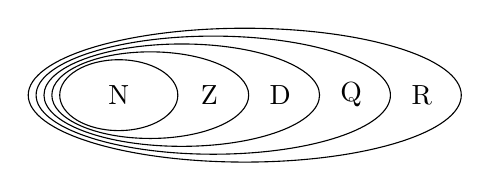
\begin{tikzpicture}
        \draw (0, 0) ellipse (0.75 and 0.45);
        \draw (0.4, 0) ellipse (1.25 and 0.55);
        \draw (0.8, 0) ellipse (1.75 and 0.65);
        \draw (1.2, 0) ellipse (2.25 and 0.75);
        \draw (1.6, 0) ellipse (2.75 and 0.85);
        \draw (0, 0) node {\mb{N}};
        \draw (1.15, 0) node {\mb{Z}};
        \draw (2.05, 0) node {\mb{D}};
        \draw (2.95, 0) node {\mb{Q}};
        \draw (3.85, 0) node {\mb{R}};
      \end{tikzpicture}
    \end{center}
    
    They are supported by a bit, a group/words (finite) of bits whose logical nature is compatible with electronic processing (on-off)
    
    \begin{center}
      \begin{tikzpicture}
        \draw (0, 0) node (hi) {0};
        \draw (0.2, 0) node {0};
        \draw (0.4, 0) node {0};
        \draw (0.6, 0) node {1};
        \draw (0.8, 0) node {0};
        \draw (1.0, 0) node {1};
        \draw (1.2, 0) node {1};
        \draw (1.4, 0) node {1};
        
        \draw (1.8, 0) node {0};
        \draw (2.0, 0) node {0};
        \draw (2.2, 0) node {0};
        \draw (2.4, 0) node {1};
        \draw (2.6, 0) node (n) {0};
        \draw (2.8, 0) node {1};
        \draw (3.0, 0) node {1};
        \draw (3.2, 0) node (e) {1};
        
        \draw (3.6, 0) node (w) {0};
        \draw (3.8, 0) node {0};
        \draw (4.0, 0) node {0};
        \draw (4.2, 0) node {1};
        \draw (4.4, 0) node {0};
        \draw (4.6, 0) node {1};
        \draw (4.8, 0) node {1};
        \draw (5.0, 0) node (b) {1};
        
        \draw (5.4, 0) node (o) {0};
        \draw (5.6, 0) node {0};
        \draw (5.8, 0) node {0};
        \draw (6.0, 0) node {1};
        \draw (6.2, 0) node {0};
        \draw (6.4, 0) node {1};
        \draw (6.6, 0) node {1};
        \draw (6.8, 0) node (low) {1};
        
        \draw[rose, thick] (b.center) ++ (-0.1, -0.2) -- ++ (0, 0.4) -- ++ (0.2, 0) -- ++ (0, -0.4) -- cycle;
        \node (bit) at ([shift={(0, 0.75)}] b) {bit};
        \draw[rose, thick] (bit.south west) ++ (0.1, 0.075) -- ++ (0.5, 0) -- ++ (0, 0.4) -- ++ (-0.5, 0) -- cycle;
        \draw[rose, thick] ([shift={(0, 0.2)}] b.center) -- ([shift={(0.35, 0.075)}] bit.south west);
        
        \node (nibble) at (2.9, 0.75) {nibble};
        \draw[bleu, thick] (2.5, -0.2) rectangle (3.3, 0.2) (2.4, 0.55) rectangle (3.4, 0.95) (2.9, 0.55) -- (2.9, 0.2);
        
        \node (lbit) at (6.8, 0.75) {Low Bit};
        \draw[thick] (6.1, 0.55) rectangle (7.5, 0.95);
        \draw[thick, ->] (6.8, 0.55) -- (6.8, 0.2);
        
        \node (hbit) at (0, 0.75) {High Bit};
        \draw[thick] (-0.75, 0.55) rectangle (0.75, 1);
        \draw[thick, ->] (0, 0.55) -- (0, 0.2);
        
        \node[anchor = west] at (5.6, -0.75) {byte};
        \draw[thick, orange] (5.3, -0.1) -- (5.3, -0.2) -- (6.9, -0.2) -- (6.9, -0.1);
        \draw[thick, orange] (5.7, -0.5) rectangle (6.5, -0.95) (5.5, -0.2) -- (5.5, -0.75) -- (5.7, -0.75);
        
        \node[anchor = west] at (3.8, -0.75) {word};
        \draw[thick, mauve] (3.5, -0.1) -- (3.5, -0.3) -- (7, -0.3) -- (7, -0.1);
        \draw[thick, mauve] (3.9, -0.55) rectangle (4.75, -0.95) (3.7, -0.3) -- (3.7, -0.75) -- (3.9, -0.75);
        
        \node[anchor = west] at (0.2, -0.75) {double word};
        \draw[thick, vertc] (-0.1, -0.1) -- (-0.1, -0.4) -- (7.1, -0.4) -- (7.1, -0.1);
        \draw[thick, vertc] (0.3, -0.55) rectangle (2.3, -0.95) (0.1, -0.4) -- (0.1, -0.75) -- (0.3, -0.75);
        
      \end{tikzpicture}
    \end{center}
    
    Representation is finite, we can only represent a subset of values : $2^n$
  \end{block}
\end{frame}

\begin{frame}{Coding numbers}
  Most of machines will offer two well known coding methods
  \begin{minipage}{0.45\textwidth}
  \begin{block}{Two’s Complement for signed integers}\small
    $$x = - b_{n-1}\times 2^{n-1} + \sum_{i = 0}^{i<n-1} b_i \times 2^i$$
    \centering

    $12_{10} - 5_{10} = 12_{10} + (-5_{10})$
    
    \begin{tabular}{c l r}
     & $0000~1100$ & $(12_{10})$\\
     $+$ & $1111~1011$ & $(5_{10})$\\\hline
     $=$ & $0000~0111$ & $(7_{10})$
    \end{tabular}
    
    \medskip
    $-2^{n-1}$\\$\rightarrow$\\$2^{n-1}-1$
  \end{block}
  \end{minipage}\hfill\begin{minipage}{0.45\textwidth}
  \begin{block}{IEEE 754 for floats}\small
    $$x = (-1)^s \times 1.m \times 2^{(e - bias)}$$
    \begin{itemize}
      \item $s$ : Sign bit (1 bit)
      \item $m$ : Mantissa (23 bits)
      \item $e$ : Exponent (8 bits)
    \end{itemize}
    
    \medskip
    \centering
    $1,175~494~35 \times 10^{−38}$\\$\rightarrow$\\$3,402~823~46 \times 10^{38}$
  \end{block}
  \end{minipage}
\end{frame}

\begin{frame}{The range problem}
  \begin{minipage}{0.35\textwidth}
  \begin{block}{}
    \begin{itemize}
      \item $2^{32} = 4,294 \times 10^9$
      \item $2^{64} = 1,844 \times 10^{19}$
      \item $2^{128} = 3,402 \times 10^{38}$
    \end{itemize}
  \end{block}
  \begin{block}{}
    \begin{itemize}
      \item $12! = 4,790 \times 10^8$
      \item $13! = 6,227 \times 10^{9}$
      \item $20! = 2,432 \times 10^{18}$
      \item $21! = 5,109 \times 10^{19}$
      \item $34! = 2,952 \times 10^{38}$
      \item $35! = 1,033 \times 10^{40}$
    \end{itemize}
  \end{block}
  \end{minipage}\hfill\begin{minipage}{0.6\textwidth}
  \begin{block}{}
    \begin{itemize}
      \item Programmer must guarantee that the integer in a specific application do not cause an overflow
      \item More and more modern applications, need to get off the range of the machine and/or of the language
      \begin{itemize}
        \item Estimated number of atoms in the observable universe $10^{80}$
        \item Earth’s mass consist of about $4\times10^{51}$ nucleons
        \item Estimated number of neuronal connections in the human brain $10^{14}$
        \item Estimated lower bound on the game-tree complexity of chess (``Shannon number") $10^{120}$
      \end{itemize}
    \end{itemize}
  \end{block}
  \end{minipage}
\end{frame}

\begin{frame}{Big numbers}
  \begin{block}{}
    \begin{itemize}
      \item Several modern programming languages have built-in or options to support for bignums : Lisp, Python, Perl, Haskell and Ruby 
      \item Others (C, C++, Java) have libraries available for arbitrary-precision integer and floating-point math
    \end{itemize}
  \end{block}
  \begin{block}{}
    Rather than store values as a fixed number of binary bits related to the size of the processor register, these implementations typically use variable-length arrays of digits 
    \begin{itemize}
      \item Reduces performances
      \item Eliminates simple overflow
      \item Guarantees the results on all machines
    \end{itemize}
  \end{block}
\end{frame}

\begin{frame}[fragile]{Exercise 1: Big addition}
  \begin{block}{Statement}
    \begin{itemize}
      \item Addition of large numbers (unsigned integers) stored in strings
      \item Numbers may be very large (may not fit in \inlc{long long int})
      \item Reads (from stdin) sequences of two strings containing big numbers
      \item Computes the sum and writes (on stdout) the string of the resulting number
      \item If one of the two input strings is not a number (\textit{i.e.} all letters of the string are not digits or the string is empty) output should be the string \inlc{"?"}
    \end{itemize}
  \end{block}
\end{frame}

\begin{frame}[fragile]{Exercise 1: Big addition}
  \begin{code}{Solution 1: Using languages with bignums}
    \begin{PseudoCode}
read $s_1$ and $s_2$ on the standard input

print $s_1 + s_2$
    \end{PseudoCode}
  \end{code}

  \begin{code}{Solution 2: Using a language \textbf{without} bignums}
    \begin{PseudoCode}
read $s_1$ and $s_2$ on the standard input

res $\leftarrow$ computes addition of $s_1$ and $s_2$

print res
    \end{PseudoCode}
  \end{code}
\end{frame}

\begin{frame}[fragile]{Exercise 1: Big addition}
  \begin{example}
    \begin{minipage}[t]{0.45\textwidth}
    \emphv{Input:}\\
    3333311111111111\\
    44422222221111\\
    \\
    4\\
    0005682\\
    0529\\
    L33T\\
    12\\
    0538\\
    2
    \end{minipage}\hfill
    \begin{minipage}[t]{0.45\textwidth}
    \emphv{Output:}\\
    3377733333332222\\
    ?\\
    6211\\
    ?\\
    540
    \end{minipage}
  \end{example}
\end{frame}

\begin{frame}[fragile]{Exercise 2: Bit Reverse}
  \begin{block}{Statement}
    Given an hexadecimal integer $x$ and a decimal integer $n$, reverse the nth lowest bit of $x$
  \end{block}
  
  \begin{block}{$n=3$}
    \begin{center}
      \begin{tabular}{*{3}{c}}
        $b_{31}\ \dots\ b_3\ 0 0 0$ & becomes & $b_{31}\ \dots\ b_3\ 0 0 0$\\
        $b_{31}\ \dots\ b_3\ 0 0 1$ & becomes & $b_{31}\ \dots\ b_3\ 1 0 0$\\
        $b_{31}\ \dots\ b_3\ 0 1 0$ & becomes & $b_{31}\ \dots\ b_3\ 0 1 0$\\
        $b_{31}\ \dots\ b_3\ 0 1 1$ & becomes & $b_{31}\ \dots\ b_3\ 1 1 0$\\
        $b_{31}\ \dots\ b_3\ 1 0 0$ & becomes & $b_{31}\ \dots\ b_3\ 0 0 1$\\
        $b_{31}\ \dots\ b_3\ 1 0 1$ & becomes & $b_{31}\ \dots\ b_3\ 1 0 1$\\
        $b_{31}\ \dots\ b_3\ 1 1 0$ & becomes & $b_{31}\ \dots\ b_3\ 0 1 1$\\
        $b_{31}\ \dots\ b_3\ 1 1 1$ & becomes & $b_{31}\ \dots\ b_3\ 1 1 1$\\
      \end{tabular}
    \end{center}
  \end{block}
  
  $\Rightarrow$ if $n \not\in [2, 32]$ $x$ is not modified
\end{frame}

\end{document}
